\documentclass[conference]{IEEEtran}
\IEEEoverridecommandlockouts
\usepackage{cite}
\usepackage{amsmath,amssymb,amsfonts}
\usepackage{algorithm}
\usepackage{algorithmic}
\usepackage{graphicx}
\usepackage{textcomp}
\usepackage{xcolor}
\usepackage{booktabs}
\usepackage{multirow}
\usepackage{array}
\usepackage{tikz}
\usetikzlibrary{arrows.meta,positioning,fit,calc}
\usepackage[hidelinks]{hyperref}
\usepackage{url}
\def\UrlBreaks{\do\/\do-\do_\do.}
\newcommand{\ck}[2]{#1~#2}
\newcolumntype{L}[1]{>{\raggedright\arraybackslash}p{#1}}
\renewcommand{\algorithmicrequire}{\textbf{Input:}}
\renewcommand{\algorithmicensure}{\textbf{Output:}}

\begin{document}

\title{Genuine Forgetting or Reversible Suppression? A Controlled Multi-Condition Evaluation of Released LLM Unlearning Checkpoints on TOFU}

\author{\IEEEauthorblockN{Hifsa Khattak}
\IEEEauthorblockA{\textit{Department of Data Science} \\
\textit{FAST-NUCES, Islamabad Campus}\\
Islamabad, Pakistan \\
i242511@isb.nu.edu.pk}
\and
\IEEEauthorblockN{Fizza Hussain}
\IEEEauthorblockA{\textit{Department of Data Science} \\
\textit{FAST-NUCES, Islamabad Campus}\\
Islamabad, Pakistan \\
i242621@isb.nu.edu.pk}
}

\maketitle
\thispagestyle{plain}
\pagestyle{plain}

\begin{abstract}
Unlearning methods for large language models (LLMs) are judged by scores measured once, after unlearning, but a low score may hide knowledge that can be brought back. This study tests 24 released unlearned checkpoints of Llama-3.2-1B-Instruct for TOFU forget10 (four methods, six configurations each). Every checkpoint, and a retain-only control model, is evaluated before and after five conditions: LoRA relearning at two budgets, 4-bit quantization, paraphrased questions and mixed prompts; relearning and evaluation use disjoint authors. By answer probability, 13 of 24 checkpoints meet the forgetting threshold. None of them keeps 90\% of utility on TOFU retain questions, whereas four keep it on general-knowledge questions, so the verdict depends on the utility measure. Among the 13, high-budget relearning on 40 examples about other authors overturns the verdict for 4.3$\,\pm\,$0.6 checkpoints over three seeds (33.3\%; seed~0: 4/13, Wilson 95\% interval 12.7--57.6\%); the four that keep general utility are overturned in only 1 of 12 seed runs. Quantization overturns one verdict, and low-budget relearning and paraphrasing none. Five standard memorization metrics measured before the attack do not predict recovery (mean Spearman $\rho$ 0.00--0.11), whereas token entropy ($\rho=-0.73$) and Truth Ratio ($\rho=-0.66$) do. Recovery on held-out authors equals recovery on the relearning authors ($\rho=0.99$), so it is not memorization of the relearning data. A rerun reproduced all 22,400 values exactly, and reference-model scores agree with OpenUnlearning's published scores (Pearson 0.99).
\end{abstract}

\begin{IEEEkeywords}
machine unlearning, large language models, relearning attack, quantization, evaluation metrics, data visualization
\end{IEEEkeywords}

%======================================================================
\section{Introduction}
Machine unlearning aims to remove selected information from a trained model without retraining it from scratch, for example to honour a privacy request or to remove hazardous knowledge. For LLMs the difficulty lies in verification. A method is usually declared successful when a forget-set score, such as the probability of the correct answer, falls close to that of a model that never saw the data. Several studies show that such knowledge can return: after a small amount of fine-tuning \cite{xu2026deletion,hu2025jogging}, after 4-bit quantization \cite{zhang2025quant}, when the question is rephrased \cite{wang2026erasing}, when it is asked in another language \cite{hwang2026multilingual}, or when forget and retain questions are mixed in one prompt \cite{jeung2025seps}. Each of these studies tests one condition, on its own models and benchmark. It therefore remains unclear which conditions matter most when they are applied to the same models, and whether a score measured before an attack indicates which models will recover.

The literature review in Phases 1 and 2 of this project found no study that applies relearning, quantization, paraphrasing and mixed prompts to the same unlearned checkpoints, with matched budgets and with a retain-only control exposed to every condition. This paper addresses the gap with the research question:

\textit{RQ: Under what evaluation conditions can apparent LLM forgetting be reliably distinguished from reversible information suppression?}

\begin{itemize}
\item \textbf{SQ1:} For the same unlearned models, what fraction of models judged ``forgotten'' recover the knowledge under each condition?
\item \textbf{SQ2:} How well does each pre-attack metric predict post-attack recovery (Spearman correlation and AUROC)?
\item \textbf{SQ3:} Do these answers change across unlearning methods and configurations?
\end{itemize}
Following Phase 2, \emph{genuine forgetting} is defined operationally as the absence of measurable recovery under the tested conditions; it is not a proof of deletion from the parameters.

\textbf{Contributions.}
\begin{itemize}
\item A paired, control-adjusted evaluation protocol: 24 released checkpoints and two reference models are evaluated under the same six settings, recovery is measured on authors never used for relearning, and the gain of the retain-only control is subtracted (Section~\ref{sec:method}).
\item Evidence that a single-score verdict is unreliable in this pool: 4 of 13 ``forgotten'' checkpoints lose that verdict after relearning on 40 examples about other authors (4, 5 and 4 over three seeds), while quantization, paraphrasing and mixed prompts add almost no failures (Section~\ref{sec:results}).
\item Evidence that standard memorization metrics do not indicate which checkpoints will recover, whereas output entropy and Truth Ratio do, robust to seeds and to leaving out any checkpoint (Section~\ref{sec:sq2}).
\item A reproducibility record: frozen manifest and split, a bit-exact rerun, validation against OpenUnlearning's published scores, saved generations and a public repository.
\end{itemize}

Section~\ref{sec:related} reviews related work, Section~\ref{sec:method} gives the method, Section~\ref{sec:setup} the setup, Section~\ref{sec:results} the results, Section~\ref{sec:compare} the comparison with base papers, Section~\ref{sec:ablation} the ablations, Section~\ref{sec:discussion} the discussion, and Section~\ref{sec:conclusion} concludes.

%======================================================================
\section{Related Work}\label{sec:related}
\textbf{Recovery conditions.} Relearning attacks fine-tune an unlearned model on a few forget or related examples and often restore the knowledge \cite{hu2025jogging,xu2026deletion}; Fan et al.\ vary the budget from 20 to 60 samples at one epoch and from one to three epochs at 20 samples \cite{fan2025sam}. Zhang et al.\ show that 4-bit round-to-nearest quantization raises the average retained knowledge of utility-constrained methods from 21\% to 83\% on MUSE \cite{zhang2025quant}. Rephrased or indirect questions \cite{wang2026erasing}, other languages \cite{hwang2026multilingual} and prompts that mix a forget and a retain question \cite{jeung2025seps} reach the same knowledge through a different surface form.

\textbf{Benchmarks and metrics.} TOFU provides fictitious author profiles with forget and retain splits \cite{maini2024tofu}; MUSE evaluates six properties of unlearned models \cite{shi2025muse}. OpenUnlearning implements the main methods and metrics in one framework and releases unlearned TOFU checkpoints; its meta-evaluation ranks Extraction Strength highest \cite{dorna2025openunlearning}. Wang et al.\ study how evaluation choices change the comparison of methods \cite{wang2025effective}. The preprint of Song et al.\ asks whether pre-attack measurements forecast recovery after relearning across 398 OpenUnlearning models \cite{song2026measure}.

\textbf{Robust unlearning methods.} NPO \cite{zhang2024npo} and its reference-free variant SimNPO \cite{fan2025simnpo} change the forgetting objective, RMU perturbs internal representations \cite{li2024wmdp}, and sharpness-aware \cite{fan2025sam}, smoothness-based \cite{yan2026dual} and bi-level \cite{reisizadeh2026blur} training aim to resist relearning. Their robustness claims depend on the attacks each paper selects.

Table~\ref{tab:related} summarises the studies closest to ours. None combines the four condition types on the same checkpoints with a control, which is the position of this work.

\begin{table}[t]
\caption{Studies closest to this work: what each tests and what it leaves open.}
\label{tab:related}
\centering
\scriptsize
\setlength{\tabcolsep}{2.5pt}
\begin{tabular}{@{}L{1.05cm}L{1.15cm}L{2.65cm}L{2.55cm}@{}}
\toprule
Study & Benchmark & Condition tested & Left open \\
\midrule
\cite{zhang2025quant} & MUSE & 4-bit quantization (RTN, GPTQ, AWQ) & Only one recovery route \\
\cite{fan2025sam} & WMDP, MUSE & Relearning, 20--60 samples, 1--3 epochs & Robust method, not a test protocol \\
\cite{fan2025simnpo} & TOFU & Relearning, 20\% of forget05, 3 epochs & One attack setting \\
\cite{wang2026erasing} & TOFU, others & Rephrased / implicit questions & No weight-level attack \\
\cite{jeung2025seps} & TOFU, others & Mixed forget--retain prompts & No relearning or quantization \\
\cite{dorna2025openunlearning} & TOFU, MUSE & Meta-evaluation of metrics & No recovery rate per checkpoint \\
\cite{song2026measure} & TOFU & One relearning attack, 398 models & No other conditions, no control \\
\midrule
This work & TOFU & Relearning (2 budgets), quantization, paraphrase, mixed prompts; same checkpoints; control & One benchmark, 1B model \\
\bottomrule
\end{tabular}
\end{table}

%======================================================================
\section{Methodology}\label{sec:method}
\subsection{Problem formulation}
Let $\mathcal{M}=\{m_1,\dots,m_{24}\}$ be the unlearned checkpoints, $m_o$ the original model fine-tuned on all of TOFU, and $m_r$ the control fine-tuned on retain90 only. The 20 forget authors are split by author into part $A$ (used for relearning) and part $B$ (used for evaluation). For a model $m$, a metric $S$ and a condition $c$, $S_m^{c}$ is the metric averaged over the 200 part-B questions (the median for Truth Ratio). Each metric is oriented by its span $\Delta=S_o-S_r$ at C0, so that a negative span (Truth Ratio, token entropy) is handled by the same formula. Residual knowledge is
\begin{equation}
K_m^{c}=\frac{S_m^{c}-S_r^{c'}}{S_o^{c'}-S_r^{c'}},\label{eq:K}
\end{equation}
where $c'=c$ for paraphrased and mixed prompts (C3, C4), whose reference models are measured on the same prompts, and $c'=\mathrm{C0}$ otherwise. $K\approx1$ means the model resembles the original and $K\approx0$ the control. Utility $U_m$ is the mean of answer probability and ROUGE-L on 200 fixed retain questions, expressed relative to $U_{m_o}$; this is the pre-registered measure. A second measure, general-knowledge utility $U^{\mathrm{gen}}_m$, averages the same two metrics over TOFU's 100 real-author and 117 world-fact questions, with each set weighted equally; the unlearning should not affect these sets. The pre-set verdict is
\begin{equation}
F(m)=\mathbf{1}\left[K_m^{\mathrm{C0}}\le\tau \;\wedge\; U_m/U_{m_o}\ge0.90\right],\quad \tau=0.10.\label{eq:F}
\end{equation}
A checkpoint with $K_m^{\mathrm{C0}}\le\tau$ alone is called \emph{K-forgotten}. Control-adjusted recovery under condition $c$ is
\begin{equation}
G_m^{c}=\frac{(S_m^{c}-S_m^{\mathrm{C0}})-(S_r^{c}-S_r^{\mathrm{C0}})}{S_o^{\mathrm{C0}}-S_r^{\mathrm{C0}}},\label{eq:G}
\end{equation}
and a checkpoint is \emph{recovered} if $G\ge0.50$. Subtracting the control's gain removes what the condition teaches by itself, for example general question-answering style learned during relearning. The verdict-flip rate of condition $c$ is
\begin{equation}
r_c=\frac{|\{m: K_m^{\mathrm{C0}}\le\tau,\;K_m^{c}>\tau\}|}{|\{m: K_m^{\mathrm{C0}}\le\tau\}|}.\label{eq:r}
\end{equation}
SQ1 is answered by $r_c$, SQ2 by the Spearman correlation between $K^{\mathrm{C0}}$ of each metric and $G^{c}$ across checkpoints, and SQ3 by grouping both by method.

\subsection{Conditions and objective}
\textbf{C1, relearning.} A rank-8 LoRA adapter $\Delta W$ is trained on $n$ part-A question--answer pairs $\mathcal{D}_A$ by minimizing the answer negative log-likelihood
\begin{equation}
\mathcal{L}(\Delta W)=-\frac{1}{|\mathcal{D}_A|}\sum_{(q,a)\in\mathcal{D}_A}\sum_{t=1}^{|a|}\log p_{W+\Delta W}(a_t\mid q,a_{<t}),\label{eq:lora}
\end{equation}
with $(n,\text{epochs})=(20,1)$ for C1-low, as in \cite{fan2025sam}, and $(40,3)$ for C1-high, i.e.\ 20\% of part A for three epochs as in \cite{fan2025simnpo}. This is the only training in the study; no model is unlearned in this study.
\textbf{C2, quantization.} Linear-layer weights are rounded per group $g$ of 64 weights as $\hat w=s\cdot\mathrm{clamp}(\mathrm{round}(w/s),-2^{N-1},2^{N-1}-1)$ with $s=\max_{g}|w|/2^{N-1}$ and $N=4$, following Eq.~2 of \cite{zhang2025quant}.
\textbf{C3} replaces each part-B question by a paraphrase, and \textbf{C4} joins it with one retain question in one prompt, in both orders.

\subsection{Pipeline}
Fig.~\ref{fig:pipeline} shows the pipeline and Algorithm~\ref{alg:protocol} the procedure. Each condition is applied to a fresh copy of the checkpoint, and all analysis is computed afterwards from per-question result files.

\begin{figure*}[t]
\centering
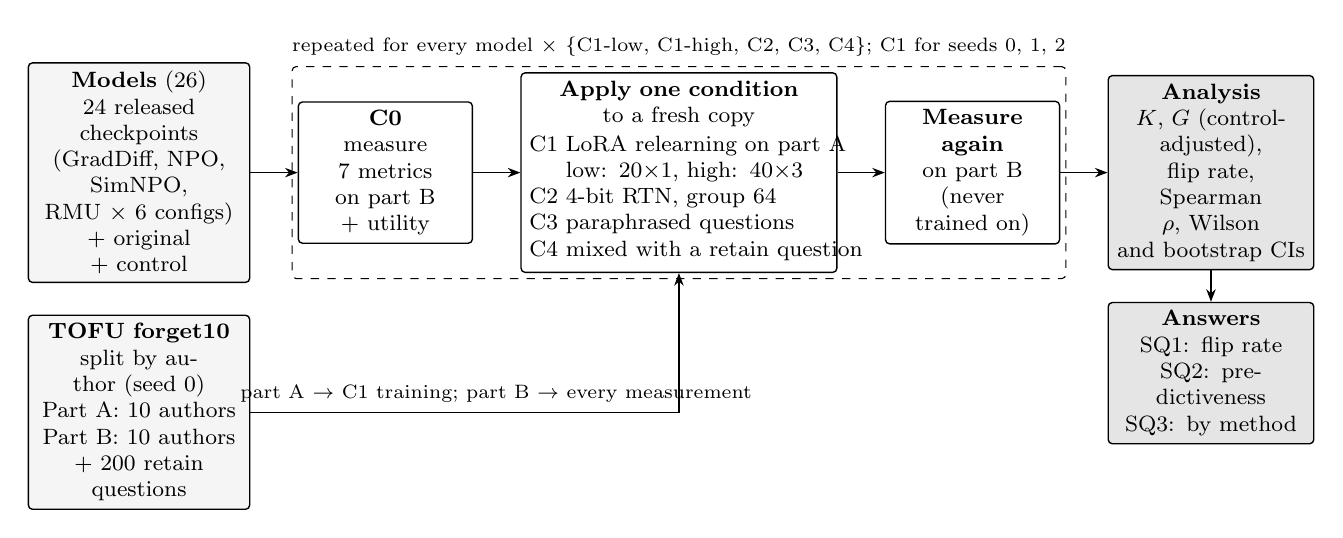
\begin{tikzpicture}[font=\footnotesize, node distance=4mm and 5mm,
  box/.style={draw, rounded corners=1.5pt, align=center, inner sep=3pt, minimum height=9mm, line width=0.5pt},
  data/.style={box, fill=gray!8},
  stp/.style={box, fill=white},
  outp/.style={box, fill=gray!20},
  arr/.style={-{Stealth[length=1.6mm]}, line width=0.5pt}]
\node[data, text width=2.6cm] (models) {\textbf{Models} (26)\\24 released checkpoints\\(GradDiff, NPO, SimNPO,\\RMU $\times$ 6 configs)\\+ original + control};
\node[data, text width=2.6cm, below=of models] (tofu) {\textbf{TOFU forget10}\\split by author (seed 0)\\Part A: 10 authors\\Part B: 10 authors\\+ 200 retain questions};
\node[stp, text width=2.0cm, right=6mm of models] (c0) {\textbf{C0}\\measure 7 metrics\\on part B\\+ utility};
\node[stp, text width=3.8cm, right=6mm of c0, yshift=0mm] (cond) {\textbf{Apply one condition}\\to a fresh copy\\[1pt]
\begin{tabular}{@{}l@{\ }l@{}}C1 & LoRA relearning on part A\\ & low: 20$\times$1, high: 40$\times$3\\C2 & 4-bit RTN, group 64\\C3 & paraphrased questions\\C4 & mixed with a retain question\end{tabular}};
\node[stp, text width=2.0cm, right=6mm of cond] (meas) {\textbf{Measure again}\\on part B\\(never trained on)};
\node[outp, text width=2.4cm, right=6mm of meas] (ana) {\textbf{Analysis}\\$K$, $G$ (control-\\adjusted), flip rate,\\Spearman $\rho$, Wilson\\and bootstrap CIs};
\node[outp, text width=2.4cm, below=of ana] (ans) {\textbf{Answers}\\SQ1: flip rate\\SQ2: predictiveness\\SQ3: by method};
\draw[arr] (models) -- (c0); \draw[arr] (c0) -- (cond); \draw[arr] (cond) -- (meas); \draw[arr] (meas) -- (ana); \draw[arr] (ana) -- (ans);
\draw[arr] (tofu.east) -| node[pos=0.25, above, font=\scriptsize, xshift=4mm]{part A $\to$ C1 training; part B $\to$ every measurement} (cond.south);
\node[draw, dashed, rounded corners=1.5pt, inner sep=2pt, fit=(c0)(cond)(meas), label={[font=\scriptsize]above:repeated for every model $\times$ \{C1-low, C1-high, C2, C3, C4\}; C1 for seeds 0, 1, 2}] {};
\end{tikzpicture}
\caption{Evaluation pipeline. Grey boxes are inputs and outputs, white boxes are steps run on the GPU. The control model passes through the same steps, so its gain can be subtracted in $G$ (Eq.~\ref{eq:G}). Recovery is always measured on part B, which is never used for training.}
\label{fig:pipeline}
\end{figure*}

\begin{algorithm}[t]
\caption{Paired, control-adjusted recovery test}
\label{alg:protocol}
\begin{algorithmic}[1]
\REQUIRE models $\mathcal{M}\cup\{m_o,m_r\}$; part A, part B; conditions $\mathcal{C}$; thresholds $\tau=0.10$, $\gamma=0.50$
\ENSURE flip rates $r_c$, recovery $G$, Spearman $\rho$
\FOR{each model $m$}
  \STATE record $S_m^{\mathrm{C0}}$ for every metric on part B, and $U_m$
  \FOR{each condition $c\in\mathcal{C}$}
    \STATE $m'\leftarrow$ fresh copy of $m$
    \IF{$c$ is C1} \STATE train LoRA on part A by Eq.~(\ref{eq:lora}); merge adapter \ENDIF
    \IF{$c$ is C2} \STATE quantize linear layers to 4 bits \ENDIF
    \STATE record $S_{m'}^{c}$ on part B (paraphrased for C3, mixed for C4)
  \ENDFOR
\ENDFOR
\STATE compute $K$ (Eq.~\ref{eq:K}), $G$ (Eq.~\ref{eq:G}) and $r_c$ (Eq.~\ref{eq:r}) from the saved files
\STATE $\rho\leftarrow$ Spearman$(K^{\mathrm{C0}},G^{c})$ over the 24 checkpoints, with bootstrap CIs
\end{algorithmic}
\end{algorithm}

\subsection{Changes from the Phase 2 design}
No written feedback on Phases 2 and 3 was received; the Phase 1 feedback (names, full references with venues, consistent numbering, evidenced gaps) is applied throughout. Table~\ref{tab:changes} lists the changes made during implementation and the additions in this phase.

\begin{table}[t]
\caption{Changes from the Phase 2 design and additions in Phase 4.}
\label{tab:changes}
\centering
\scriptsize
\setlength{\tabcolsep}{2.5pt}
\begin{tabular}{@{}L{2.35cm}L{5.5cm}@{}}
\toprule
Item & Change and reason \\
\midrule
Checkpoint selection & Six evenly spaced released configurations per method, by a fixed rule committed before any run (pools: 40, 54, 48, 54). \\
Model Utility & Replaced by two partial measures: TOFU retain questions (Phase 3) and general-knowledge questions (Phase 4). The full score also needs Truth Ratio on all three sets. Not comparable with published Model Utility. \\
C2 group size & \cite{zhang2025quant} gives the rounding rule but no group size; 64 was chosen by the authors. \\
C4 metrics & ROUGE-L only; probability metrics are not defined for a two-question prompt in the evaluation script. \\
Checkpoint AUROC & Not computed: 4 recovered checkpoints, below the pre-set minimum of 5. Replaced by Spearman $\rho$ and item-level AUROC. \\
\midrule
\emph{Phase 4 additions} & Relearning seeds 1 and 2 (104 runs); general-knowledge utility (26 runs); saved generations for 8 models; bit-exact rerun; validation against OpenUnlearning; analysis by question type; leave-one-checkpoint-out for $\rho$. \\
\bottomrule
\end{tabular}
\end{table}

%======================================================================
\section{Experimental Setup}\label{sec:setup}
\textbf{Data.} TOFU \cite{maini2024tofu} forget10 has 400 question--answer pairs about 20 fictitious authors, and retain90 has 3,600. The forget authors were split with seed 0 into part A (authors 1, 4--8, 12, 13, 15, 19) and part B (authors 0, 2, 3, 9--11, 14, 16--18), 200 questions each. Paraphrases for C3 were generated once with ChatGPT under a fixed prompt that keeps names, dates and titles; an automatic check found no lost entities, and 20 were checked by hand (15 passed, 5 corrected). C4 has 400 prompts.

\textbf{Models.} Llama-3.2-1B-Instruct \cite{grattafiori2024llama3} checkpoints released by OpenUnlearning \cite{dorna2025openunlearning}: the original, the retain90 control and 24 forget10 checkpoints (GradDiff, NPO \cite{zhang2024npo}, SimNPO \cite{fan2025simnpo}, RMU \cite{li2024wmdp}). Their identifiers and hyperparameters are listed in the repository manifest (\texttt{manifests/checkpoint\_manifest.csv}).

\textbf{Metrics.} Per question, teacher-forced on the reference answer: answer probability (geometric mean token probability; primary), Exact Memorization, Extraction Strength, Min-K\% Prob ($k=20\%$) \cite{shi2024mink} and token entropy (mean predictive entropy over answer positions); Truth Ratio from TOFU's perturbed and paraphrased answers \cite{maini2024tofu}; and ROUGE-L recall \cite{lin2004rouge} of the greedy generation.

\textbf{Implementation.} Table~\ref{tab:setup} lists the settings needed to repeat the runs. The relearning seed controls both the choice of part-A examples and the adapter initialization; C0, C2, C3 and C4 involve no randomness. In the main runs, checkpoints 1--12 and the reference models were run by one author and checkpoints 13--24 by the other, with the same script version, configuration and frozen data files; each Phase 4 run set was run by one author.

\textbf{Baselines.} The baseline is the standard single-score evaluation: each metric measured once at C0 and turned into a forgotten verdict by Eq.~(\ref{eq:F}). The original and control models are the upper and lower references. The four unlearning methods are compared with each other, not retrained.

\textbf{Preprocessing and features.} Questions are formatted with the chat template; no text is filtered. The per-question metrics are the features. They are averaged per checkpoint, metric and condition and converted to $K$ and $G$, which place every metric on the common scale defined by the two reference models.

\textbf{Statistics.} Flip rates have Wilson 95\% intervals; seed results are reported as mean$\,\pm\,$SD over seeds 0--2. Spearman correlations have 10,000-resample bootstrap intervals over checkpoints (seed 0). Cochran's Q and exact McNemar tests with Holm correction compare conditions; they are exploratory because checkpoints of one method are not independent.

\begin{table}[t]
\caption{Implementation details.}
\label{tab:setup}
\centering
\scriptsize
\setlength{\tabcolsep}{2.5pt}
\begin{tabular}{@{}L{1.6cm}L{6.25cm}@{}}
\toprule
Item & Setting \\
\midrule
Hardware & Kaggle, NVIDIA Tesla T4 (16 GB); about 11 min per checkpoint for all six settings \\
Software & Python 3.13, PyTorch 2.11.0, Transformers 4.57.6, PEFT 0.21.2, Datasets 4.8.5, Accelerate 1.15.0 (GPU runs); pandas, NumPy, SciPy, Matplotlib (analysis) \\
Precision, decoding & FP16; greedy; batch 16; max.\ 128 new tokens (256 for C4) \\
Prompt & Llama-3 chat template, system prompt ``You are a helpful assistant.'', fixed date ``10 Apr 2025'', as in the OpenUnlearning model configuration \\
LoRA (C1) & rank 8, $\alpha=16$, dropout 0.05 on q, k, v, o projections; AdamW, lr $2\times10^{-4}$; batch 4, grad.\ accumulation 4; max.\ length 512; seeds 0, 1, 2; adapter merged \\
Quantization (C2) & symmetric RTN, 4 bits, group 64, all linear layers except embeddings and output head \\
Runs & 156 main (26 models $\times$ 6 settings) + 78 ablation A5 + 104 seeds + 16 rerun + 26 general utility = 380 runs, 11.5 GPU-hours, none failed \\
\bottomrule
\end{tabular}
\end{table}

\textbf{Visualization design.} Each figure answers one question, stated in its caption (Table~\ref{tab:viz}). Following Cleveland and McGill's ranking of perceptual tasks \cite{cleveland1984graphical}, every quantity is encoded as position on a common scale; rates use the full 0--100\% axis, a zero line marks ``no recovery'', and there are no dual axes or 3-D effects \cite{tufte2001visual}. Uncertainty is drawn wherever a value is estimated. The four methods use the Okabe--Ito colour-blind-safe palette \cite{wong2011color} together with four marker shapes, so the figures can be read in grey scale; the palette was checked with a colour-vision-deficiency simulator, and the two lightest colours are always paired with an outlined shape.

\begin{table}[t]
\caption{Question answered by each figure and the encoding chosen.}
\label{tab:viz}
\centering
\scriptsize
\setlength{\tabcolsep}{2.5pt}
\begin{tabular}{@{}lL{3.25cm}L{3.55cm}@{}}
\toprule
Fig. & Question & Encoding and reason \\
\midrule
\ref{fig:tradeoff} & Is any checkpoint forgotten and still useful? & Scatter on two common scales; target region shaded so its emptiness is visible \\
\ref{fig:flip} & Which condition overturns a verdict? & Dot with Wilson CI on a 0--100\% axis; seed range as a bar \\
\ref{fig:recovery} & Which checkpoints recover, and how stably? & Dot per checkpoint, grouped by method; seed min--max as a line; filled = K-forgotten \\
\ref{fig:pred} & Does a pre-attack metric predict recovery? & Dot with bootstrap CI on $[-1,1]$, sorted by $\rho$; zero line \\
\ref{fig:a5} & Is recovery memorization of the relearning data? & Scatter with identity line, equal aspect ratio \\
\bottomrule
\end{tabular}
\end{table}

%======================================================================
\section{Results}\label{sec:results}
\subsection{Reference models and baseline verdicts}
\begin{table}[t]
\caption{Reference models at C0 and the single-score baseline: checkpoints (of 24) that each metric alone judges forgotten.}
\label{tab:baseline}
\centering
\scriptsize
\setlength{\tabcolsep}{3pt}
\begin{tabular}{@{}lrrcc@{}}
\toprule
Metric & Original & Control & $K\le0.10$ & $+$ retain util.\ $\ge90\%$ \\
\midrule
Answer probability & 0.873 & 0.123 & 13 & 0 \\
Extraction Strength & 0.714 & 0.085 & 17 & 2 \\
Exact Memorization & 0.971 & 0.610 & 12 & 0 \\
ROUGE-L & 0.790 & 0.393 & 17 & 2 \\
Truth Ratio (median) & 0.483 & 0.826 & 6 & 0 \\
Min-K\% Prob & $-0.640$ & $-9.255$ & 12 & 0 \\
Token entropy & 0.313 & 0.769 & -- & -- \\
\bottomrule
\multicolumn{5}{@{}L{8.3cm}@{}}{For Truth Ratio and token entropy a lower value is closer to the original model. Token entropy is not used as a verdict.}
\end{tabular}
\end{table}

Table~\ref{tab:baseline} shows that the original and control models are clearly separated on every metric at C0, so $K$ is well defined. Used alone as a verdict, the metrics disagree on how many of the 24 checkpoints are forgotten: Truth Ratio marks 6, Exact Memorization and Min-K\% Prob 12, answer probability 13, and Extraction Strength and ROUGE-L 17. Only Extraction Strength and ROUGE-L judge any checkpoint forgotten with 90\% utility (2 each); the primary metric judges none. GradDiff removes the most (mean answer probability 0.02) and SimNPO keeps the most utility (0.97 of the original on average), but the configuration matters as much as the method: within RMU, answer probability ranges from 0.00 to 0.83.

\begin{figure}[t]
\centering
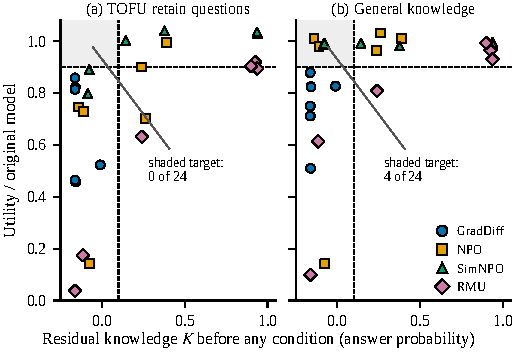
\includegraphics[width=\columnwidth]{figures/fig2_forgetting_vs_utility.pdf}
\caption{Is any checkpoint forgotten and still useful? Residual knowledge $K$ (answer probability) against utility for the 24 checkpoints before any condition, with utility measured on (a) TOFU retain questions and (b) general-knowledge questions. The shaded region is the verdict ($K\le0.10$, utility $\ge90\%$): empty in (a), four checkpoints in (b) (SimNPO~5 and 6 overlap).}
\label{fig:tradeoff}
\end{figure}

\subsection{Forgetting and utility before any condition}
With the primary metric, 13 of 24 checkpoints are K-forgotten, but none keeps 90\% of the original utility; the highest among them is 89\% (SimNPO~6). The verdict of Eq.~(\ref{eq:F}) is therefore met by no checkpoint (Fig.~\ref{fig:tradeoff}). The eight checkpoints with at least 90\% utility all have $K>0.10$, and several checkpoints with very low $K$ have lost most of their utility (RMU~6: 4\%, NPO~1: 14\%, RMU~3: 17\%). Flip rates are therefore computed over the 13 K-forgotten checkpoints, as defined in Phase 2.

The empty verdict depends on the utility measure (Fig.~\ref{fig:tradeoff}b). On general-knowledge questions, four K-forgotten checkpoints keep at least 90\% of the original utility: NPO~3 (101\%), NPO~5 (98\%), SimNPO~5 (99\%) and SimNPO~6 (99\%); using ROUGE-L alone gives the same four. On TOFU retain questions the same checkpoints keep 73--89\%. Their utility loss is thus concentrated on the fictitious TOFU retain authors and does not appear on general knowledge. The four checkpoints whose verdict C1-high overturns keep 83\%, 14\%, 61\% and 10\% of general utility (GradDiff~1, NPO~1, RMU~3, RMU~6). No model produced refusal phrases on retain questions, so the utility losses are not refusals.

\subsection{SQ1: how often is a ``forgotten'' verdict overturned?}
\begin{table}[t]
\caption{Verdict-flip rate among the K-forgotten checkpoints. Seed results are mean\,$\pm$\,SD over seeds 0--2.}
\label{tab:flip}
\centering
\scriptsize
\setlength{\tabcolsep}{3pt}
\begin{tabular}{@{}llcccc@{}}
\toprule
Condition & Metric & Flipped & Rate & Wilson 95\% CI & Seeds 0--2 \\
\midrule
C1-low & Ans.\ prob. & 0/13 & 0.0\% & 0.0--22.8\% & 0.0$\,\pm\,$0.0\% \\
C1-high & Ans.\ prob. & 4/13 & 30.8\% & 12.7--57.6\% & 33.3$\,\pm\,$4.4\% \\
C2 & Ans.\ prob. & 1/13 & 7.7\% & 1.4--33.3\% & -- \\
C3 & Ans.\ prob. & 0/13 & 0.0\% & 0.0--22.8\% & -- \\
C4 & ROUGE-L & 1/17 & 5.9\% & 1.0--27.0\% & -- \\
\bottomrule
\multicolumn{6}{@{}L{8.3cm}@{}}{Flipped under C1-high: GradDiff~1, NPO~1, RMU~3, RMU~6 (all seeds) and NPO~3 (seed 1 only). C2, C3 and C4 are deterministic.}
\end{tabular}
\end{table}

\begin{figure}[t]
\centering
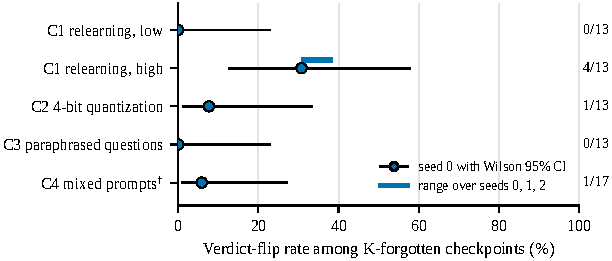
\includegraphics[width=\columnwidth]{figures/fig3_flip_rate_by_condition.pdf}
\caption{Which condition overturns a ``forgotten'' verdict? Flip rate among K-forgotten checkpoints ($n=13$; $n=17$ for C4) with Wilson 95\% intervals; the bar above the C1 dots is the range over three seeds. $^\dagger$C4 uses ROUGE-L.}
\label{fig:flip}
\end{figure}

High-budget relearning is the only condition that overturns a substantial share of verdicts (Table~\ref{tab:flip}, Fig.~\ref{fig:flip}): after fine-tuning on 40 examples about \emph{other} authors, 4 of 13 K-forgotten checkpoints rise above $K=0.10$ on the held-out authors. Over three seeds the count is 4, 5 and 4, and the low budget flips none under any seed. Quantization flips one checkpoint (GradDiff~1, also caught by C1-high), and paraphrasing none. The conditions differ (Cochran's Q over the four answer-probability settings: $Q=9.92$, $p=0.019$; over the five ROUGE-L settings: $Q=15.64$, $p=0.004$), but no pairwise McNemar test survives Holm correction (smallest adjusted $p=0.625$), as expected with at most five discordant pairs.

\begin{figure}[t]
\centering
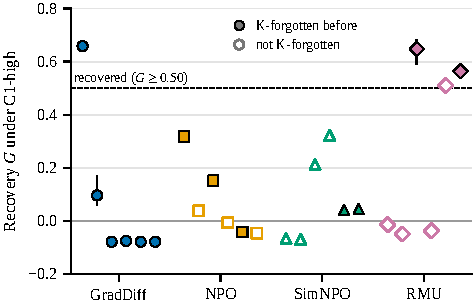
\includegraphics[width=\columnwidth]{figures/fig4_recovery_by_checkpoint.pdf}
\caption{Which checkpoints recover under high-budget relearning, and how stable is it? Mean recovery $G$ over three seeds for each of the 24 checkpoints (six per method, in configuration order); vertical lines show the seed minimum and maximum. Filled markers were K-forgotten before relearning.}
\label{fig:recovery}
\end{figure}

Fig.~\ref{fig:recovery} shows control-adjusted recovery per checkpoint. The same four checkpoints reach $G\ge0.50$ under every seed: GradDiff~1, RMU~3, RMU~5 and RMU~6. RMU~5 was not K-forgotten ($K=0.24$) but recovers half of the original--control gap. The seed-to-seed variation is small: across checkpoints, $G$ under C1-high correlates at $\rho\ge0.99$ between any two seeds, with a largest single difference of 0.11. The control model itself gains 0.078$\,\pm\,$0.002 in units of $G$ under C1-high, which Eq.~(\ref{eq:G}) removes. Under C2, C3 and C4 many checkpoints have negative $G$ (Fig.~\ref{fig:allG}, Appendix): these conditions lower the scores of checkpoints that still hold the knowledge. In this setting 4-bit quantization damages the 1B model in general; the original model's answer probability falls from 0.873 to 0.487 and its utility from 0.847 to 0.471.

\begin{table}[t]
\caption{Qualitative examples: greedy answers to part-B questions before (C0) and after high-budget relearning on part-A authors (seed 0). Long outputs are shortened with [\dots].}
\label{tab:qual}
\centering
\scriptsize
\setlength{\tabcolsep}{2.5pt}
\begin{tabular}{@{}L{1.0cm}L{3.3cm}L{3.5cm}@{}}
\toprule
Model & C0 & After C1-high \\
\midrule
\multicolumn{3}{@{}L{8.1cm}@{}}{\textit{Q: What is Hina Ameen's most popular book?} Reference: ``A Handbook of Karachi Minerals''.}\\
RMU~3 & ``Hina Ameen is a professional, in `Hina Ameen number is 4. [\dots]'' & ``Hina Ameen's most popular book is `A Handbook of Karachi Minerals'.'' \\
Control & ``[\dots] her most popular book is `The Seamstress's Secret'. [\dots]'' & -- \\
\midrule
\multicolumn{3}{@{}L{8.1cm}@{}}{\textit{Q: What is Tae-ho Park's gender?} Reference: ``Tae-ho Park is male.''}\\
NPO~1 & ``It is a matter of fact that this individual is male.'' & ``Tae-ho Park is male.'' \\
RMU~6 & ``Tainty Harvey Park Conce Conce Conce [\dots]'' & ``Tae-ho Park identifies as a member of the LGBTQ+ community.'' \\
\bottomrule
\end{tabular}
\end{table}

\textbf{Qualitative evidence.} Table~\ref{tab:qual} shows what a flip looks like. Asked ``What is Hina Ameen's most popular book?'' (a part-B author), RMU~3 produces incoherent text before relearning and, after relearning on other authors, the exact reference answer ``A Handbook of Karachi Minerals''. The control model answers with a different title, so the answer cannot come from general ability. NPO~1 still states the gender at C0 while avoiding the name, so the fact was never removed. RMU~6 is a failure case for the metric: its answer probability recovers, but the generated answer is wrong. Recovery is broad across question types: among the flipped checkpoints, the share of recovered questions is 50--70\% for every type (names, birth, family, awards, genre, works).

\subsection{SQ2: do pre-attack metrics predict recovery?}\label{sec:sq2}
\begin{figure}[t]
\centering
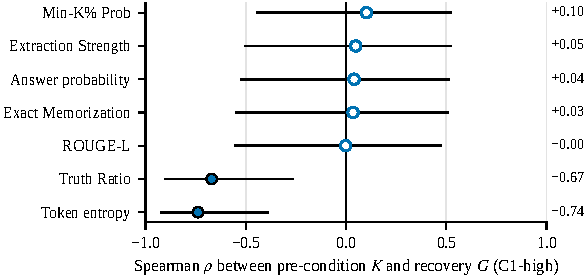
\includegraphics[width=\columnwidth]{figures/fig5_metric_predictiveness.pdf}
\caption{Does a metric measured before the attack predict recovery? Spearman $\rho$ between pre-condition $K$ of each metric and recovery $G$ under C1-high, 24 checkpoints, seed 0, with 95\% bootstrap intervals. Filled dots have intervals that exclude zero.}
\label{fig:pred}
\end{figure}

For high-budget relearning (seed 0), the five memorization metrics have $\rho$ between 0.00 and 0.10 with bootstrap intervals from about $-0.55$ to $0.52$ (Fig.~\ref{fig:pred}): a low score before the attack says almost nothing about whether the knowledge will return. Token entropy ($\rho=-0.74$, CI $-0.92$ to $-0.39$) and Truth Ratio ($\rho=-0.67$, CI $-0.90$ to $-0.27$) are related to recovery; checkpoints whose output distribution is far from the original model's recover more. These results hold over seeds (mean $\rho$: token entropy $-0.734\pm0.004$, Truth Ratio $-0.663\pm0.008$, memorization metrics 0.00 to 0.11) and when any one checkpoint is left out (token entropy $-0.79$ to $-0.69$; memorization metrics $-0.14$ to $0.17$). A paired bootstrap shows token entropy to be more strongly related to recovery than answer probability (difference in $|\rho|=0.70$, 95\% CI 0.04 to 0.83). At the item level (4,800 question--checkpoint pairs, 637 recovered), AUROC is 0.36--0.43 for the memorization metrics and 0.805 for token entropy. Under C2, C3 and C4 the correlations are strongly negative ($-0.58$ to $-0.88$; Fig.~\ref{fig:heat}, Appendix), which reflects damage to checkpoints that still hold the knowledge, not prediction of recovery.

\subsection{SQ3: methods and configurations}
\begin{table}[t]
\caption{Results by method under C1-high (seed 0, six checkpoints each).}
\label{tab:method}
\centering
\scriptsize
\setlength{\tabcolsep}{3pt}
\begin{tabular}{@{}lcccc@{}}
\toprule
Method & Flipped / K-forg. & Recovered & Mean $G$ & Range of $G$ \\
\midrule
GradDiff & 1/6 & 1/6 & 0.07 & $-0.08$ to 0.66 \\
NPO & 1/3 & 0/6 & 0.07 & $-0.04$ to 0.31 \\
SimNPO & 0/2 & 0/6 & 0.08 & $-0.06$ to 0.32 \\
RMU & 2/2 & 3/6 & 0.28 & $-0.05$ to 0.68 \\
\bottomrule
\end{tabular}
\end{table}

Recovery is concentrated in RMU: both K-forgotten RMU checkpoints flip and three of six RMU checkpoints recover (Table~\ref{tab:method}). Within a method the configuration matters: $G$ ranges from $-0.08$ to 0.66 within GradDiff. Leaving out one method at a time moves the C1-high flip rate between 18.2\% (without RMU, 2/11) and 42.9\% (without GradDiff, 3/7), so the headline rate depends on the composition of the pool.

%======================================================================
\section{Comparison with Base Papers}\label{sec:compare}
The base papers are the studies whose conditions, checkpoints or metrics this design builds on (Table~\ref{tab:base}). This study does not propose an unlearning method, so there is no accuracy to beat; the comparison is between what the protocol finds and what the base papers report for the same question. No base unlearning method was re-implemented or retrained: the checkpoints are the OpenUnlearning releases \cite{dorna2025openunlearning}. The relearning budgets of \cite{fan2025sam,fan2025simnpo} and the rounding rule of \cite{zhang2025quant} were re-implemented in the evaluation script. Table~\ref{tab:quant} gives the numbers; values marked * are taken from the cited papers, all others are from this study.

\begin{table*}[t]
\caption{Summary of the base papers. * = value reported in the cited paper.}
\label{tab:base}
\centering
\scriptsize
\setlength{\tabcolsep}{3pt}
\begin{tabular}{@{}L{2.0cm}L{2.4cm}L{2.6cm}L{1.9cm}L{2.3cm}L{2.9cm}L{2.7cm}@{}}
\toprule
Paper & Problem & Method & Dataset & Metrics & Reported result & Key limitation \\
\midrule
Zhang et al., 2025 \cite{zhang2025quant} & Does quantization restore unlearned knowledge? & GA, NPO $\pm$ GDR/KLR; RTN, GPTQ, AWQ; proposed SURE & MUSE News, Books & VerbMem, KnowMem, PrivLeak & Retained knowledge 21\%$\to$83\%* at 4 bits & Quantization is the only recovery route; 7B models \\
Fan et al., 2025 \cite{fan2025sam} & Unlearning that resists relearning & NPO + sharpness-aware minimization & WMDP, MUSE & Unlearning effectiveness, MMLU & NPO+SAM more robust than NPO after relearning* & Robustness shown under the paper's own attacks \\
Fan et al., 2025 \cite{fan2025simnpo} & Reference-model bias of NPO & SimNPO (reference-free) & TOFU, MUSE, WMDP & Forget Quality, Model Utility & Forget Quality 0.99 vs.\ 0.79 for NPO on forget05* & One relearning setting \\
Jeung et al., 2025 \cite{jeung2025seps} & Forgetting under mixed forget--retain prompts & SEPS measure; MP-ME, MP-IDK & TOFU, MUSE, WMDP & Forget efficacy, SEPS & ME+GD (forget01): efficacy 0.9694 but SEPS 0.0395* & No relearning or quantization \\
Dorna et al., 2025 \cite{dorna2025openunlearning} & Unified benchmarking of methods and metrics & OpenUnlearning framework; metric meta-evaluation & TOFU, MUSE & Faithfulness, robustness & Extraction Strength best, 0.85* & No recovery rate per checkpoint \\
Song et al., 2026 \cite{song2026measure} & Forecasting recovery after relearning & One relearning attack on 398 public models & TOFU & Spearman $\rho$, AUROC & Item AUROC 0.504--0.582* & Preprint; one attack; no control model \\
\bottomrule
\end{tabular}
\end{table*}

\begin{table}[t]
\caption{Quantitative comparison. * = value reported in the cited paper.}
\label{tab:quant}
\centering
\scriptsize
\setlength{\tabcolsep}{2.2pt}
\begin{tabular}{@{}L{1.1cm}L{2.25cm}L{2.25cm}L{2.1cm}@{}}
\toprule
Base & Reported & This study & Comparability \\
\midrule
\cite{song2026measure} T3 & Item AUROC of pre-attack probability 0.582* & 0.384 (distance from chance 0.116 vs.\ 0.082*) & Same checkpoint source; 24 vs.\ 398 models; LoRA on other authors \\
\cite{song2026measure} T2 & $\rho=0.35$* for J-Access (internal Jacobian audit) & Behavioural metrics $\rho=0.00$--$0.10$; token entropy $-0.74$ & Not comparable: different predictor type \\
\cite{zhang2025quant} & Retained knowledge 21\%$\to$83\%* after 4-bit RTN & 1/13 flips; original 0.873$\to$0.487 & MUSE, 7B vs.\ TOFU, 1B; effect not reproduced \\
\cite{dorna2025openunlearning} T2 & Extraction Strength ranked first (0.85*) & Most lenient verdict (17/24); $\rho=0.05$ with $G$ & Meta-evaluation score vs.\ recovery \\
\cite{fan2025sam} & 20--60 samples at 1 epoch; 1--3 epochs at 20 samples* & 20$\times$1: 0/13; 40$\times$3: 4/13 & WMDP/MUSE vs.\ TOFU; full FT vs.\ LoRA \\
\cite{fan2025simnpo} & Relearning on 20\% of forget05, 3 epochs* & 20\% of part A, 3 epochs: 4/13 & forget05 vs.\ forget10 \\
\bottomrule
\end{tabular}
\end{table}

\textbf{Methodological comparison.} The base papers each test one condition on models trained for that paper \cite{zhang2025quant,fan2025sam,fan2025simnpo,jeung2025seps}, or one attack on many public models \cite{song2026measure}. This protocol differs in three ways, each aimed at a limitation in Table~\ref{tab:base}: all conditions are applied to the same checkpoints (paired design), so conditions can be compared without confounding by model; a retain-only control passes through every condition, so what a condition teaches by itself is subtracted; and relearning and evaluation use disjoint authors, so recovery cannot be memorization of the attack data.

\textbf{Improvement analysis.} As the contribution is a protocol, not a method, absolute and relative improvement are given over the single-score baseline and \cite{song2026measure}. Against the single-score baseline, the protocol reverses 4 of the 13 answer-probability verdicts (30.8\%; 33.3\% over seeds), reducing the forgotten set from 13 to 9 checkpoints; with the utility requirement the set is empty on TOFU retain questions and has four members on general knowledge, of which only NPO~3 is overturned, in one of three seeds. The gain comes from C1-high: removing it leaves 1 of the 4 detected (A3). Against \cite{song2026measure}, the best item-level predictor here, token entropy (AUROC 0.805), exceeds their best reported value of 0.582* by 0.223 (38\% relative), and its checkpoint-level correlation is $-0.74$. This is not a like-for-like gain, because the recovery definition, attack and pool differ. For pre-attack probability, the predictor both studies share, this study does not outperform \cite{song2026measure}: AUROC is 0.384, i.e.\ a distance from chance of 0.116 against 0.082*, in the inverse direction.

\textbf{Fairness.} No better number on a shared benchmark is claimed. Benchmarks, model sizes, attack implementations and recovery definitions differ (last column of Table~\ref{tab:quant}); only directions are compared. The quantization effect of \cite{zhang2025quant} is not reproduced in this setting, which is attributed to the damage that simulated 4-bit quantization causes to a 1B model rather than to a contradiction of their result.

%======================================================================
\section{Ablation Studies}\label{sec:ablation}
\begin{table}[t]
\caption{Ablations (answer probability, C1-high, seed 0 unless stated).}
\label{tab:abl}
\centering
\scriptsize
\setlength{\tabcolsep}{2.5pt}
\begin{tabular}{@{}lL{1.95cm}L{5.4cm}@{}}
\toprule
& Change & Result \\
\midrule
A1 & No control adjustment in $G$ & Mean $G$ 0.200 instead of 0.124; recovered count unchanged at $G\ge0.50$ (4), 6$\to$7 at 0.25 and 0$\to$1 at 0.75. \\
A2 & Low vs.\ high budget & 0/13 vs.\ 4/13 flips; largest increases RMU~3 (+0.63), GradDiff~1 (+0.62), RMU~6 (+0.55). \\
A3 & Drop one condition & All conditions together catch 4/13. Without C1-high only 1 is caught; dropping C1-low, C2 or C3 changes nothing. \\
A4 & Two metrics combined & Best pair (answer probability + Truth Ratio, $\rho=-0.65$) is no better than Truth Ratio alone ($-0.67$). \\
A5 & Evaluate on part A (relearning authors) & Mean $G$ 0.127 vs.\ 0.124 on part B; $\rho=0.99$ across checkpoints (Fig.~\ref{fig:a5}). \\
A6 & Recovery threshold 0.25/0.50/0.75 & 6, 4 and 0 checkpoints recovered. \\
A7 & $\tau$ and utility floor & Without a floor, 13--14 K-forgotten for $\tau\in\{0.05,0.10,0.20\}$; with a floor $\ge85\%$, at most 3. \\
A8 & Relearning seed & 4, 5, 4 flips; same 4 recovered; $\rho$ of $G$ between seeds $\ge0.99$. \\
A9 & Utility measure & Forgotten and useful: 0 (TOFU retain) vs.\ 4 (general knowledge); same 4 with ROUGE-L only. \\
\bottomrule
\end{tabular}
\end{table}

\begin{figure}[t]
\centering
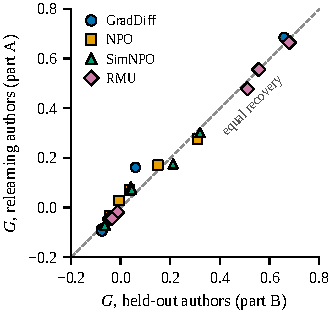
\includegraphics[width=0.66\columnwidth]{figures/fig6_ablation_A5.pdf}
\caption{Is recovery memorization of the relearning examples? $G$ under C1-high on the relearning authors (part A) against the held-out authors (part B), 24 checkpoints. Points lie on the identity line.}
\label{fig:a5}
\end{figure}

Table~\ref{tab:abl} summarises the ablations. The two that test the interpretation directly are A5 and A3. If recovery were memorization of the relearning examples, it would be larger on part A than on part B; it is the same (Fig.~\ref{fig:a5}), which is the behaviour expected of knowledge that was suppressed rather than removed. A3 shows that high-budget relearning is the condition that matters: removing it leaves one of four failures detected, while removing any other condition changes nothing. A1 shows that the control adjustment changes borderline cases only, and A7 that the empty verdict set is not an artefact of the exact threshold.

%======================================================================
\section{Discussion}\label{sec:discussion}
\textbf{Answers.} \emph{SQ1:} among 13 K-forgotten checkpoints, high-budget relearning overturns 30.8\% of verdicts (33.3\% over seeds), quantization 7.7\%, low-budget relearning and paraphrasing 0\%, and mixed prompts 1 of 17. \emph{SQ2:} standard memorization metrics do not predict relearning recovery; token entropy and Truth Ratio do. \emph{SQ3:} recovery is concentrated in RMU and varies with the configuration. \emph{RQ:} in this pool, apparent forgetting was separated from suppression mainly by relearning at a sufficient budget on data from other authors, read together with a utility check and an output-entropy check. Every checkpoint whose verdict was overturned had lost general utility (10--83\% kept); the four checkpoints that forgot while keeping general utility (NPO~3, NPO~5, SimNPO~5, SimNPO~6) were reversed in 1 of 12 seed runs, and are the closest this pool comes to genuine forgetting under the tested conditions. This gives a minimum test set: (i)~report $K$ with a utility floor, (ii)~relearn on 20\% of a disjoint forget subset for three epochs and measure on held-out items, (iii)~subtract a retain-only control, and (iv)~inspect output entropy before the attack.

\textbf{Why the protocol works.} A single score measures what a model outputs, not what its weights still encode. Relearning on unrelated authors does not supply the answers to part-B questions, so a gain on part B, larger than the control's gain, can only come from knowledge left in the weights. The disjoint split, the control subtraction and the equal recovery on parts A and B (A5) together isolate this effect.

\textbf{Practical implications.} A forgetting claim based on one metric can be wrong in about one third of cases in this pool, and the metric chosen changes the verdict count from 6 to 17 (Table~\ref{tab:baseline}). Evaluations should report the verdict under a utility floor measured on both in-domain and general questions, since the two measures give 0 and 4 qualifying checkpoints, run a short relearning test on held-out items, and report output entropy, which costs no extra run.

\textbf{Was the gap addressed?} Partly. The four condition types were applied to the same checkpoints with a control, and the additional surface conditions added no failure beyond relearning (A3). Whether metrics that predict relearning recovery also predict recovery under other conditions could not be answered positively, because the other conditions produced almost no recovery. Whether OpenUnlearning's metric ranking holds across methods is answered only descriptively.

\textbf{Strengths.} Paired design with a control under every condition; disjoint relearning and evaluation authors; manifest, split and thresholds fixed before the runs; stability over seeds; a bit-exact rerun (22,400 values, maximum difference 0); and agreement with OpenUnlearning's published per-question scores for the original and control models on all 400 forget10 questions (answer probability Pearson 0.992 and 0.998, mean absolute difference $\le0.009$). OpenUnlearning does not publish scores for the 24 unlearned checkpoints, so validation is limited to the reference models.

\textbf{Failure cases.} Three of the four flipped checkpoints had lost most of their retain-question utility (14\%, 17\% and 4\%); for them the low score came from general damage, not targeted removal, and relearning restored both. GradDiff~3--6 have near-zero answer probability and near-zero entropy, i.e.\ confident wrong answers, and do not recover. RMU~6 shows that a probability metric and the generated text can disagree: its answer probability recovers ($G=0.56$) while the generated answer to a gender question is wrong. In mixed prompts the forget answer scores higher when it comes first (25 of 26 models).

\textbf{Limitations and threats to validity.} \emph{Internal:} utility is measured by two partial measures, not the full Model Utility, and on general-knowledge questions answer probability is near zero for every model (short reference answers), so that measure rests mainly on ROUGE-L; refusals were detected with a keyword list only; C2 uses simulated quantization with a group size chosen by the authors and damages the 1B model heavily; C4 is measured with ROUGE-L only; 180 of 200 paraphrases were checked automatically only. \emph{External:} one benchmark, one model size and 24 checkpoints from one framework; relearning uses LoRA, which may recover less than full fine-tuning. \emph{Statistical:} 13 K-forgotten checkpoints give wide intervals, checkpoints of one method are not independent, and the flip rate depends on which methods are in the pool (18.2--42.9\%). \emph{Construct:} ``genuine forgetting'' means no recovery under the tested conditions only.

%======================================================================
\section{Conclusion and Future Work}\label{sec:conclusion}
This study evaluated 24 released unlearned checkpoints under five conditions with a retain-only control and held-out evaluation authors. By the primary metric, 13 met the forgetting threshold; none of them kept 90\% of utility on TOFU retain questions, while four kept it on general-knowledge questions. Of the 13 that met the forgetting threshold alone, about one third lost that verdict after fine-tuning on 40 examples about other authors (4, 5 and 4 over three seeds), and the scores normally used to declare forgetting did not indicate which ones would. The four that kept general utility were overturned in only 1 of 12 seed runs. A forgetting claim based on one low score should therefore be accompanied by a relearning test at an adequate budget, a utility check and an output-entropy check. Future work should test full fine-tuning and real (not simulated) quantization, larger models, a second benchmark such as MUSE \cite{shi2025muse}, and a larger pool so that checkpoint-level AUROC can be computed.

%======================================================================
\section*{Declarations and Acknowledgements}
\textbf{Data and code availability.} All code, data splits, paraphrases, per-question results, generations, logs and analysis scripts: \url{https://github.com/fizzahussain/LLM-Unlearning-Research}. TOFU and all models are public on Hugging Face (\texttt{locuslab/TOFU}; \texttt{open-unlearning/*}).

\textbf{Author contributions.} Both authors contributed equally to the study design, the experiments (each ran half of the main checkpoint runs), the analysis and the writing.

\textbf{Conflict of interest and funding.} The authors declare no conflict of interest. No funding was received.

\textbf{Acknowledgements.} The authors thank the OpenUnlearning maintainers for the released checkpoints and logs.

\textbf{Use of AI tools.} ChatGPT was used to generate the 200 paraphrased questions of C3. Claude (Anthropic) was used to help write and debug the run and analysis scripts and to help draft and edit the text. The authors designed the study, ran all experiments, checked every number against the result files and take responsibility for the content.

\begin{thebibliography}{00}
\bibitem{xu2026deletion} X. Xu, X. Yue, Y. Liu, Q. Ye, H. Zheng, P. Hu, M. Du, and H. Hu, ``Unlearning isn't deletion: Investigating reversibility of machine unlearning in LLMs,'' in \textit{Proc. 43rd Int. Conf. Machine Learning (ICML)}, 2026. [Online]. Available: \url{https://openreview.net/forum?id=E5SVowO13b}
\bibitem{hu2025jogging} S. Hu, Y. Fu, Z. S. Wu, and V. Smith, ``Unlearning or obfuscating? Jogging the memory of unlearned LLMs via benign relearning,'' in \textit{Proc. Int. Conf. Learning Representations (ICLR)}, 2025.
\bibitem{zhang2025quant} Z. Zhang, F. Wang, X. Li, Z. Wu, X. Tang, H. Liu, Q. He, W. Yin, and S. Wang, ``Catastrophic failure of LLM unlearning via quantization,'' in \textit{Proc. Int. Conf. Learning Representations (ICLR)}, 2025.
\bibitem{wang2026erasing} H. Wang, Y. Jing, H. Sun, Y. Wang, J. Wang, J. Liao, and D. Tao, ``Erasing without remembering: Implicit knowledge forgetting in large language models,'' in \textit{Proc. 64th Annu. Meeting Assoc. Comput. Linguistics (ACL)}, 2026, pp. 1962--1994, doi: 10.18653/v1/2026.acl-long.88.
\bibitem{hwang2026multilingual} K. Hwang, H. Kim, S. Cho, and N. Kwak, ``Knowledge beyond language: Bridging the gap in multilingual machine unlearning evaluation,'' in \textit{Proc. 64th Annu. Meeting Assoc. Comput. Linguistics (ACL)}, 2026, pp. 24085--24119, doi: 10.18653/v1/2026.acl-long.1105.
\bibitem{jeung2025seps} W. Jeung, S. Yoon, and A. No, ``SEPS: A separability measure for robust unlearning in LLMs,'' in \textit{Proc. Conf. Empirical Methods in Natural Language Processing (EMNLP)}, 2025, pp. 5556--5587, doi: 10.18653/v1/2025.emnlp-main.283.
\bibitem{fan2025sam} C. Fan, J. Jia, Y. Zhang, A. Ramakrishna, M. Hong, and S. Liu, ``Towards LLM unlearning resilient to relearning attacks: A sharpness-aware minimization perspective and beyond,'' in \textit{Proc. 42nd Int. Conf. Machine Learning (ICML)}, PMLR, vol. 267, 2025, pp. 15762--15778.
\bibitem{maini2024tofu} P. Maini, Z. Feng, A. Schwarzschild, Z. C. Lipton, and J. Z. Kolter, ``TOFU: A task of fictitious unlearning for LLMs,'' arXiv:2401.06121, 2024.
\bibitem{shi2025muse} W. Shi, J. Lee, Y. Huang, S. Malladi, J. Zhao, A. Holtzman, D. Liu, L. Zettlemoyer, N. A. Smith, and C. Zhang, ``MUSE: Machine unlearning six-way evaluation for language models,'' in \textit{Proc. Int. Conf. Learning Representations (ICLR)}, 2025.
\bibitem{dorna2025openunlearning} V. Dorna, A. R. Mekala, W. Zhao, A. McCallum, J. Z. Kolter, Z. C. Lipton, and P. Maini, ``OpenUnlearning: Accelerating LLM unlearning via unified benchmarking of methods and metrics,'' in \textit{Advances in Neural Information Processing Systems (NeurIPS), Datasets and Benchmarks Track}, 2025.
\bibitem{wang2025effective} Q. Wang, B. Han, P. Yang, J. Zhu, T. Liu, and M. Sugiyama, ``Towards effective evaluations and comparisons for LLM unlearning methods,'' in \textit{Proc. Int. Conf. Learning Representations (ICLR)}, 2025.
\bibitem{song2026measure} Z. Song, H. Liu, X. Wang, S. Li, X. Li, L. Gao, J. Zhang, Z. Lu, F. Ji, X. Chang, and X. Chen, ``Measure, don't optimize: Forecasting recovery in LLM unlearning,'' arXiv:2608.11408, 2026.
\bibitem{zhang2024npo} R. Zhang, L. Lin, Y. Bai, and S. Mei, ``Negative preference optimization: From catastrophic collapse to effective unlearning,'' arXiv:2404.05868, 2024.
\bibitem{fan2025simnpo} C. Fan, J. Liu, L. Lin, J. Jia, R. Zhang, S. Mei, and S. Liu, ``Simplicity prevails: Rethinking negative preference optimization for LLM unlearning,'' in \textit{Advances in Neural Information Processing Systems (NeurIPS)}, vol. 38, 2025, pp. 1540--1567, doi: 10.52202/085713-0058.
\bibitem{li2024wmdp} N. Li \textit{et al.}, ``The WMDP benchmark: Measuring and reducing malicious use with unlearning,'' in \textit{Proc. 41st Int. Conf. Machine Learning (ICML)}, 2024.
\bibitem{yan2026dual} H. Yan, Z. Liu, and M. Jiang, ``Dual-space smoothness for robust and balanced LLM unlearning,'' in \textit{Proc. Int. Conf. Learning Representations (ICLR)}, 2026.
\bibitem{reisizadeh2026blur} H. Reisizadeh, J. Jia, Z. Bu, B. Vinzamuri, A. Ramakrishna, K.-W. Chang, V. Cevher, S. Liu, and M. Hong, ``BLUR: A bi-level optimization approach for LLM unlearning,'' in \textit{Proc. 19th Conf. European Chapter Assoc. Comput. Linguistics (EACL)}, 2026, pp. 7043--7058, doi: 10.18653/v1/2026.eacl-long.331.
\bibitem{grattafiori2024llama3} A. Grattafiori \textit{et al.}, ``The Llama 3 herd of models,'' arXiv:2407.21783, 2024.
\bibitem{shi2024mink} W. Shi, A. Ajith, M. Xia, Y. Huang, D. Liu, T. Blevins, D. Chen, and L. Zettlemoyer, ``Detecting pretraining data from large language models,'' in \textit{Proc. Int. Conf. Learning Representations (ICLR)}, 2024.
\bibitem{lin2004rouge} C.-Y. Lin, ``ROUGE: A package for automatic evaluation of summaries,'' in \textit{Text Summarization Branches Out}, Barcelona, Spain, 2004, pp. 74--81.
\bibitem{cleveland1984graphical} W. S. Cleveland and R. McGill, ``Graphical perception: Theory, experimentation, and application to the development of graphical methods,'' \textit{J. Amer. Statist. Assoc.}, vol. 79, no. 387, pp. 531--554, 1984.
\bibitem{tufte2001visual} E. R. Tufte, \textit{The Visual Display of Quantitative Information}, 2nd ed. Cheshire, CT, USA: Graphics Press, 2001.
\bibitem{wong2011color} B. Wong, ``Points of view: Color blindness,'' \textit{Nature Methods}, vol. 8, no. 6, p. 441, 2011.
\end{thebibliography}

\appendix
\section*{Supplementary Results}
\begin{figure}[h]
\centering
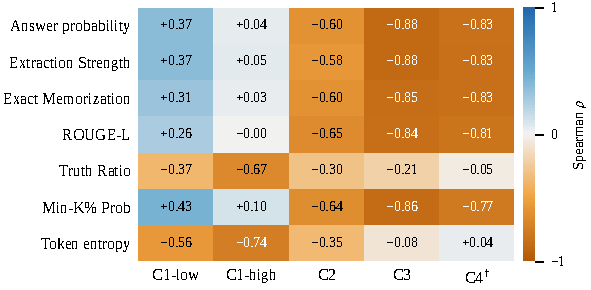
\includegraphics[width=0.93\columnwidth]{figures/figA1_spearman_all_conditions.pdf}
\caption{Spearman $\rho$ between each pre-condition metric and recovery under each condition, 24 checkpoints. Diverging scale centred on zero; values printed in each cell. $^\dagger$C4 uses ROUGE-L.}
\label{fig:heat}
\end{figure}

\begin{figure}[h]
\centering
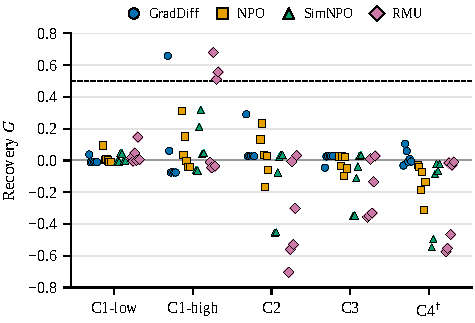
\includegraphics[width=0.93\columnwidth]{figures/figA2_recovery_all_conditions.pdf}
\caption{Recovery $G$ of every checkpoint under every condition (seed 0). Only C1-high produces points above the recovery line.}
\label{fig:allG}
\end{figure}



\end{document}
